\chapter{Implementace}

Tato kapitola popisuje implementaci dokumentace a komponent.

\section{Struktura logiky}\label{section:structure}

Všechna logika komponenty je zapouzdřena v primitivní funkci.
Tato funkce nese název \texttt{create*}, kde \texttt{*} je název komponenty.
Komponenty mají většinou podobnou signaturu funkce, která vrací objekt s následujícími \textit{properties}:

\begin{itemize}
    \item \textbf{props} --- objekt s ARIA a \gls{html} atributy a \textit{event listeners}.
    \item \textbf{state} --- stav komponenty, většinou se jedná o vnitřní stav komponenty, který chceme vystavit uživateli komponenty.
    \item \textbf{reference} --- některé komponenty potřebují referenci na přímý \gls{html} element, který se v Solid.js předává pomocí proměnných\footnote{\url{https://solidjs.com/tutorial/bindings_refs}} a direktiv\footnote{\url{https://solidjs.com/tutorial/bindings_directives}}.
\end{itemize}

Některé komponenty (například \fr{SpinButton}) mají více \gls{html} elementů na které je potřeba navázat ARIA atributy a event listeners, proto jejich funkce vrací více \textbf{props} properties (například buttonProps, rootProps).
Při více \textbf{props} properties je potřeba navázat danou property na odpovídající \gls{html} element, který je zmíněn v dokumentaci.

Koncový uživatel tuto primitivní funkci zavolá v definici komponenty a předá jí všechny potřebné argumenty.
Manuálně naváže \textbf{props} na \gls{html} elementy, předá potřebné \textbf{reference} a využije \textbf{state} pro vykreslení stavu komponenty.
Výhodou tohoto přístupu z kapitoly~\ref{technology:dist} je, že vývojář má absolutní kontrolu nad \gls{html} strukturou komponenty a použitým CSS řešením.
\clearpage

\begin{listing}[!ht]
    \begin{minted}{jsx}
import { createExample } from "lib"

export const Example = (args) => {
    const {
        rootProps,
        buttonProps,
        state
    } = createExample(args)!\mintedlabel{docs-page-example-9}!

    return (
        <div {...rootProps}>!\mintedlabel{docs-page-example-12}!
            <button {...buttonProps}>Toggle</button>!\mintedlabel{docs-page-example-13}!
            {state.isVisible ? <p>Content</p> : null}!\mintedlabel{docs-page-example-14}!
        </div>
    )
}
\end{minted}
    \caption{Příklad implementace komponenty pomocí primitivní funkce}
    \label{implementation-example}
\end{listing}

Na ukázce~\ref{implementation-example} je příklad použití primitivní funkce \texttt{createExample} pro vytvoření komponenty \texttt{Example}.
Řádek~\ref{docs-page-example-9} zavolá primitivní funkci a předá jí argumenty, které jsou definovány v \texttt{ExampleArgs}.
Elementům na řádku~\ref{docs-page-example-12} a~\ref{docs-page-example-13} jsou předány atributy a event listeners pomocí spread operátoru.
Na řádku~\ref{docs-page-example-14} je ukázka využití vnitřního stavu komponenty pro vykreslení obsahu.

\subsection{Adresářová struktura}

Každá komponenta má svůj adresář, který obsahuje všechny soubory týkající se její implementace:

\vspace{11pt}

\dirtree{%
    .1 example.
    .2 \textbf{example.spec.ts} (jednotkové testy).
    .2 \textbf{example.ts} (logika komponenty).
    .2 \textbf{index.ts} (barrel export z types.ts a example.ts).
    .2 \textbf{types.ts} (definice typů pro komponentu).
}

\vspace{11pt}

Soubor \texttt{index.ts} slouží pro export všech položek ze souborů \texttt{types.ts} a \texttt{example.ts} pro usnadnění distribuce.
Tato technika se nazývá \textit{barrel} export.

\clearpage

\section{Disclosure}

Požadavek na klávesovou navigaci \hyperref[ofr11]{\fr{OFR 1.1}} a otevírání/zavírání obsahu \hyperref[dfr11]{\fr{DFR 1.1}} je splněn pomocí primitivní funkce \texttt{createDisclosure}.

Příkladová implementace komponenty Disclosure pomocí primitivní funkce \texttt{createDisclosure} je možná vidět na ukázce~\ref{disclosure-example}.

\subsection{Parametry}

Funkce má jeden parametr, kterým je objekt s následujícími properties:

\begin{table}[ht]\label{table:disclosure-params}
    \begin{ctucolortab}
        \begin{tabularx}{\textwidth}{X X X}
            \bfseries Název             & \bfseries Datový typ & \bfseries Výchozí hodnota \\\Midrule{}
            \texttt{defaultVisible}     & \texttt{boolean}     & \texttt{false}            \\
            \texttt{id}                 & \texttt{string}      & ---                       \\
            \texttt{isButtonElement}    & \texttt{boolean}     & \texttt{true}             \\
            \texttt{isVisible}          & \texttt{boolean}     & ---                       \\
            \texttt{onVisibilityChange} & \texttt{Function}    & ---
        \end{tabularx}
    \end{ctucolortab}
    \caption{Parametry funkce createDisclosure}
\end{table}

Z ukázky kódu~\ref{disclosure-controlled-vs-uncontrolled} je patrné, že \texttt{isVisible} a \texttt{onVisibilityChange} properties slouží pro řízení stavu komponenty z vnějšku (komponenta typu controlled), jinak je komponenta uncontrolled.
Pro případ uncontrolled komponent slouží property \texttt{defaultVisible} pro změnu výchozího zobrazení obsahu.

Property \texttt{isButtonElement} je určena pro případ, kdy element pro otevírání a zavírání obsahu není \texttt{button} a je potřeba přidat správnou ARIA roli a další atributy pro správnou interpretaci odečítači obrazovky.

V neposlední řadě property \texttt{id} slouží pro definování vlastního identifikátoru elementu s obsahem.
Ve výchozím stavu je identifikátor generován automaticky pomocí \texttt{createUniqueId}\footnote{\url{https://docs.solidjs.com/reference/component-apis/create-unique-id}}.

\clearpage

\subsection{Návratová hodnota}

Tato funkce vrací objekt s properties \texttt{toggleProps}, \texttt{contentProps} a \texttt{state}.

\begin{table}[ht]\label{table:disclosure-return}
    \begin{ctucolortab}
        \begin{tabularx}{\textwidth}{p{3cm} X}
            \bfseries Název       & \bfseries Popis                                                     \\\Midrule{}
            \texttt{contentProps} & Event listeners, atributy pro element držící obsah Disclosure.      \\
            \texttt{state}        & Vnitřní stav komponenty.                                            \\
            \texttt{toggleProps}  & Event listeners, atributy pro tlačítko pro otevření/zavření obsahu.
        \end{tabularx}
    \end{ctucolortab}
    \caption{Návratová hodnota funkce createDisclosure}
\end{table}

\subsection{ARIA atributy}

Požadavek \hyperref[ofr12]{\fr{OFR 1.2}} u Disclosure komponenty vynucuje následující atributy:

\begin{table}[ht]\label{table:disclosure-aria}
    \begin{ctucolortab}
        \begin{tabularx}{\textwidth}{X X X}
            \bfseries Název        & \bfseries Objekt     & \bfseries Typ \\\Midrule{}
            \texttt{aria-expanded} & \texttt{toggleProps} & Stav          \\
            \texttt{aria-controls} & \texttt{toggleProps} & Vlastnost
        \end{tabularx}
    \end{ctucolortab}
    \caption{Použité ARIA atributy pro Disclosure komponentu}
\end{table}

Stavový atribut \texttt{aria-expanded}\footnote{\url{https://w3.org/TR/wai-aria/\#aria-expanded}} určuje, zda je obsah otevřený nebo zavřený a vlastnost \texttt{aria-controls}\footnote{\url{https://w3.org/TR/wai-aria/\#aria-controls}} určuje, který element je ovládán tlačítkem.

\clearpage

\section{SpinButton}

Požadavky \hyperref[sfr11]{\fr{SFR 1.1}} a \hyperref[sfr12]{\fr{SFR 1.2}} jsou splněny pomocí primitivní funkce\\ \texttt{createSpinButton}.

Příkladová implementace komponenty SpinButton pomocí primitivní funkce \texttt{createSpinButton} je možná vidět na ukázce~\ref{spinbutton-example}.

\subsection{Parametry}

Funkce má jeden parametr, kterým je objekt s následujícími properties:

\begin{table}[ht]\label{table:spinbutton-params}
    \begin{ctucolortab}
        \begin{tabularx}{\textwidth}{X X X}
            \bfseries Název   & \bfseries Datový typ & \bfseries Výchozí hodnota \\\Midrule{}
            \texttt{values *} & \texttt{T[]}         & ---                       \\
            \texttt{mapping}  & \texttt{string[]}    & ---                       \\
            \texttt{step}     & \texttt{number}      & 1
        \end{tabularx}
    \end{ctucolortab}
    \caption{Parametry funkce createSpinButton}
\end{table}

Property \texttt{values} je pole hodnot generického typu, který ale musí být typu \texttt{number}, nebo \texttt{string}.
Může se stát situace, kdy hodnoty ve \texttt{values} nemají sémantický význam, proto jejich význam je možné definovat v property \texttt{mapping}.

Poslední property \texttt{step} určuje o kolik se má hodnota zvýšit, nebo snížit při stisknutí kláves \texttt{PageUp} a \texttt{PageDown}.

\subsection{Návratová hodnota}

Tato funkce vrací objekt s properties \texttt{inputProps}, \texttt{decrementButtonProps}, \texttt{incrementButtonProps} a \texttt{state}.

\begin{table}[ht]\label{table:spinbutton-return}
    \begin{ctucolortab}
        \begin{tabularx}{\textwidth}{p{5cm} X}
            \bfseries Název               & \bfseries Popis                                           \\\Midrule{}
            \texttt{decrementButtonProps} & Event listeners a atributy pro tlačítko snižující hodnotu \\
            \texttt{incrementButtonProps} & Event listeners a atributy pro tlačítko zvyšující hodnotu \\
            \texttt{inputProps}           & Event listeners a atributy pro vstupní pole.              \\
            \texttt{state}                & Vnitřní stav komponenty.
        \end{tabularx}
    \end{ctucolortab}
    \caption{Návratová hodnota funkce createSpinButton}
\end{table}

\clearpage

\subsection{ARIA atributy}

Požadavek \hyperref[ofr12]{\fr{OFR 1.2}} u SpinButton komponenty vynucuje následující atributy:

\begin{table}[ht]
    \begin{ctucolortab}
        \begin{tabularx}{\textwidth}{X X X}
            \bfseries Název         & \bfseries Objekt    & \bfseries Typ \\\Midrule{}
            \texttt{role}           & \texttt{inputProps} & Role          \\
            \texttt{aria-valuenow}  & \texttt{inputProps} & Vlastnost     \\
            \texttt{aria-valuemin}  & \texttt{inputProps} & Vlastnost     \\
            \texttt{aria-valuemax}  & \texttt{inputProps} & Vlastnost     \\
            \texttt{aria-valuetext} & \texttt{inputProps} & Vlastnost     \\
            \texttt{aria-invalid}   & \texttt{inputProps} & Stav
        \end{tabularx}
    \end{ctucolortab}
    \caption{Použité ARIA atributy pro SpinButton komponentu}
    \label{table:spinbutton-aria}
\end{table}

Role je nastavena na \texttt{"spinbutton"}.
Vlastnost \texttt{aria-valuenow}\footnote{\url{https://w3c.github.io/aria/\#aria-valuenow}} definuje momentální index hodnoty komponenty a spolupracuje synergicky s atributem \texttt{aria-valuetext}\footnote{\url{https://w3c.github.io/aria/\#aria-valuetext}}, který definuje textovou podobu hodnoty.

Dvě důležité vlastnosti \texttt{aria-valuemin}\footnote{\url{https://w3c.github.io/aria/\#aria-valuemin}} a \texttt{aria-valuemax}\footnote{\url{https://w3c.github.io/aria/\#aria-valuemax}} definují minimální, respektive maximální hodnotu, kterou může komponenta nabývat.

Stavový atribut \texttt{aria-invalid}\footnote{\url{https://w3c.github.io/aria/\#aria-invalid}} definuje zda je hodnota vstupního pole validní, tedy zda se nachází v hodnotách z pole \texttt{values}.

\clearpage

\section{Toolbar}

Stěžejní logikou komponenty \fr{Toolbar} je klávesová navigace.
Zásadní je správné chování focusu, které jsem přejal z knihovny React Aria, které má robustní řešení s ohledem na různé druhy prohlížečů a kombinace odečítačů obrazovky.

Přejaté soubory jsou popsané níže:

\begin{itemize}
    \item \textbf{dom-helpers.ts} --- Pomocné funkce pro získání správného \texttt{ownerWindow} a \texttt{ownerDocument} objektů z \gls{dom}.
    \item \textbf{focus-safely.ts} --- Funkce pro přesun focusu na element bez vedlejších efektů pro odečítače obrazovky.
    \item \textbf{focus-without-scrolling.ts} --- Funkce pro přesun focusu na element bez posunu stránky.
    \item \textbf{focus.ts} --- Funkce pro přesun focusu v rámci elementu.
    \item \textbf{interactions.ts} --- Kód, který detekuje jakým způsobem uživatel interaguje se stránkou (klávesnice, dotek, nebo virtualizované klikání)
    \item \textbf{is-element-visible.ts} --- Funkce kontrolující zda je daný element viditelný.
    \item \textbf{is-virtual-click.ts} --- Funkce detekující virtuální klikání.
    \item \textbf{live-announcer.ts} --- Třída \texttt{LiveAnnouncer}, která přidává neviditelné elementy do \gls{dom} s oznámením změn pro odečítače obrazovky.
    \item \textbf{platform.ts} --- Funkce pro detekci platformy na kterém běží kód. Slouží pro případnou korekci chování v různých prohlížečích.
    \item \textbf{run-after-transition.ts} --- Funkce, která zavolá callback funkci jakmile skončí všechny přechody v rámci stránky.
\end{itemize}

Samotná implementace komponenty exportuje funkci \texttt{createToolbar} a její použití pro implementaci komponenty Toolbar je možná vidět na ukázce~\ref{toolbar-example}.

\clearpage

\subsection{Parametry}

První parametr je objekt pro konfiguraci Toolbaru s následujícími properties:

\begin{table}[ht]
    \begin{ctucolortab}
        \begin{tabularx}{\textwidth}{X X X}
            \bfseries Název          & \bfseries Datový typ               & \bfseries Výchozí hodnota \\\Midrule{}
            \texttt{orientation}     & \texttt{"horizontal" | "vertical"} & \texttt{"horizontal"}     \\
            \texttt{aria-labelledby} & \texttt{string}                    & ---                       \\
            \texttt{aria-label}      & \texttt{string}                    & ---
        \end{tabularx}
    \end{ctucolortab}
    \caption{Parametry createToolbar funkce}
    \label{table:toolbar-params}
\end{table}

Parametr \texttt{orientation} slouží pro splnění požadavku \hyperref[tfr12]{\fr{TFR 1.2}} a určuje jaké klávesy slouží pro navigaci v Toolbaru.
Pokud je nastaveno \texttt{"horizontal"}, tak šipky vlevo a vpravo přesunou focus mezi focusovatelnými prvky v rámci Toolbaru.
U hodnoty \texttt{"vertical"} se používají šipky nahoru a dolů.

Parametry \texttt{aria-labelledby}\footnote{\url{https://w3.org/TR/wai-aria/\#aria-labelledby}} a \texttt{aria-label}\footnote{\url{https://w3.org/TR/wai-aria/\#aria-label}} slouží pro pojmenování instance komponenty a splnění tak požadavku \href{ofr13}{\fr{OFR 1.3}}.

Druhým parametrem funkce je nepovinná Solid.js reference na kořenový element Toolbaru.
Pokud není reference předána, tak je možné ji získat pomocí Solid.js direktivy \texttt{use:toolbarRef}, která je navrácena z volání funkce \texttt{createToolbar}.

\subsection{Návratová hodnota}

Tato funkce vrací objekt s properties \texttt{toolbarProps} a nepovinně \texttt{toolbarRef}.

\begin{table}[ht]\label{table:toolbar-return}
    \begin{ctucolortab}
        \begin{tabularx}{\textwidth}{p{3cm} X}
            \bfseries Název       & \bfseries Popis                                              \\\Midrule{}
            \texttt{toolbarProps} & Event listeners, atributy pro element držící obsah Toolbaru. \\
            \texttt{toolbarRef}   & Solid.js direktiva pro předání reference na HTML element.
        \end{tabularx}
    \end{ctucolortab}
    \caption{Návratová hodnota funkce createToolbar}
\end{table}

\clearpage

\subsection{ARIA atributy}

Požadavek \hyperref[ofr12]{\fr{OFR 1.2}} u Toolbar komponenty vynucuje následující atributy:

\begin{table}[ht]\label{table:toolbar-aria}
    \begin{ctucolortab}
        \begin{tabularx}{\textwidth}{X X X}
            \bfseries Název           & \bfseries Objekt      & \bfseries Typ \\\Midrule{}
            \texttt{role}             & \texttt{toolbarProps} & Role          \\
            \texttt{aria-label}       & \texttt{toolbarProps} & Vlastnost     \\
            \texttt{aria-labelledby}  & \texttt{toolbarProps} & Vlastnost     \\
            \texttt{aria-orientation} & \texttt{toolbarProps} & Vlastnost
        \end{tabularx}
    \end{ctucolortab}
    \caption{Použité ARIA atributy pro Toolbar komponentu}
\end{table}

Role je nastavena na \texttt{"toolbar"}, aby odečítače obrazovky správně interpretovali element jako Toolbar komponentu.
Pokud je v rámci Toolbaru vnořený jiný Toolbar, tak role vnitřního Toolbaru je nastavena na \texttt{"group"}.
Vlastnost \texttt{aria-orientation}\footnote{\url{https://w3.org/TR/wai-aria/\#aria-orientation}} je nastavena dle hodnoty argumentu \texttt{orientation}, obdobně pro vlastnosti \texttt{aria-label} a \texttt{aria-labelledby}.

\section{Tooltip}

Pro implementaci Tooltipu bylo využito následujících primitiv ze Solid Aria knihovny:

\begin{itemize}
    \item \textbf{createFocusable} --- Vytvoří z elementu focusovatelný element.
    \item \textbf{createFocusVisible} --- Sleduje jakým zařízení uživatel interaguje se stránkou a podle toho rozhoduje, zda má být viditelný focus.
    \item \textbf{createHover} --- Normalizuje \textit{hover} interakci napříč prohlížeči a dotykovými zařízeními.
    \item \textbf{createInteractionModality} --- Sleduje jakým zařízení uživatel interaguje se stránkou.
    \item \textbf{createOverlayTriggerState} --- Vytvoří booleovský stav pro zobrazení obsahu.
\end{itemize}

Logika této komponenty vychází z React Aria implementace a celkově jě rozdělena do tří funkcí.
Jejich použití pro implementaci komponenty Tooltip je možné vidět na ukázce~\ref{tooltip-example}.

\clearpage

\subsection{createTooltipTriggerState}

První funkce slouží pro správu stavu Tooltipu.
Zároveň tato funkce spravuje globální stav všech otevřených Tooltipů tak, aby vždy byl otevřený jenom jeden z nich.
Také se stará o rychlost zavírání a otevírání obsahu Tooltipu.

Ze Solid Aria knihovny byla využita funkce \texttt{createOverlayTriggerState}.
Jedná se o jednoduchou funkci, která vytváří booleovský stav.
Na tuto funkci byla navázána vlastní logika pro správu globálního stavu otevření Tooltipů a časování otevírání obsahu.

\subsubsection{Parametry}

Tato funkce má jeden parametr, kterým je objekt s následujícími properties:

\begin{table}[ht]\label{table:tooltip-trigger-state-params}
    \begin{ctucolortab}
        \begin{tabularx}{\textwidth}{X X X}
            \bfseries Název       & \bfseries Datový typ & \bfseries Výchozí hodnota \\\Midrule{}
            \texttt{closeDelay}   & \texttt{number}      & \texttt{500}              \\
            \texttt{defaultOpen}  & \texttt{boolean}     & ---                       \\
            \texttt{delay}        & \texttt{number}      & 1500                      \\
            \texttt{isOpen}       & \texttt{false}       & ---                       \\
            \texttt{onOpenChange} & \texttt{Function}    & ---
        \end{tabularx}
    \end{ctucolortab}
    \caption{Parametry createTooltipTriggerState funkce}
\end{table}

Properties \texttt{closeDelay} a \texttt{delay} určují rychlost zavírání, respektive otevírání obsahu Tooltipu.
Pro případ, kdy uživatel chce měnit stav Tooltipu z vnějšího prostředí (controlled), tak lze použít properties \texttt{isOpen} a \texttt{onOpenChange}.
Pokud uživatel nechává interní stav komponenty, tak je možné použít property \texttt{defaultOpen} pro nastavení výchozího stavu otevření.

\subsubsection{Návratová hodnota}

Tato funkce vrací jeden objekt s properties \texttt{open}, \texttt{close} a \texttt{isOpen}.

\begin{table}[ht]\label{table:tooltip-trigger-state-return}
    \begin{ctucolortab}
        \begin{tabularx}{\textwidth}{p{3cm} X}
            \bfseries Název & \bfseries Popis                             \\\Midrule{}
            \texttt{close}  & Callback funkce pro zavření tooltipu.       \\
            \texttt{isOpen} & Proměnná indikující stav otevření tooltipu. \\
            \texttt{open}   & Callback funkce pro otevření tooltipu.
        \end{tabularx}
    \end{ctucolortab}
    \caption{Návratová hodnota funkce createTooltipTriggerState}
\end{table}

\subsection{createTooltipTrigger}

Druhá funkce slouží pro vytvoření elementu s ARIA atributy a event listeners pro který se má zobrazit Tooltip obsah.

Ze Solid Aria knihovny jsou využity funkce \texttt{createInteractionModality}, \texttt{createFocusable}, \texttt{createHover} a \texttt{createFocusVisible}.

\subsubsection{Parametry}

Tato funkce má dva parametry.
První parametr je objekt s properties v tabulce \ref{table:tooltip-trigger-params}.
Druhý parametr je Solid.js reference na element, který má zobrazit Tooltip.

\begin{table}[ht]
    \begin{ctucolortab}
        \begin{tabularx}{\textwidth}{X X X}
            \bfseries Název     & \bfseries Datový typ         & \bfseries Výchozí hodnota \\\Midrule{}
            \texttt{isDisabled} & \texttt{boolean}             & \texttt{false}            \\
            \texttt{trigger}    & \texttt{"focus" | undefined} & ---
        \end{tabularx}
    \end{ctucolortab}
    \caption{Parametry createTooltipTrigger funkce}
    \label{table:tooltip-trigger-params}
\end{table}

Property \texttt{isDisabled} slouží pro deaktivaci Tooltipu, když je nastavena na \texttt{true}, tak Tooltip se nikdy nezobrazí.
Property \texttt{trigger} určuje na jaký typ interakce se má Tooltip zobrazit.
Ve výchozím režimu se Tooltip otevírá při hover i focus interakci.
Při nastavení hodnoty \texttt{"focus"} se Tooltip otevírá pouze při focus interakci jinak se otevírá při všech výše zmíněných interakcích.

\subsubsection{Návratová hodnota}

Tato funkce vrací objekt s properties \texttt{tooltipProps} a \texttt{triggerProps}.

\begin{table}[ht]
    \begin{ctucolortab}
        \begin{tabularx}{\textwidth}{p{3cm} X}
            \bfseries Název       & \bfseries Popis                                                           \\\Midrule{}
            \texttt{tooltipProps} & Event listeners, atributy pro element držící obsah Tooltipu.              \\
            \texttt{triggerProps} & Event listeners, atributy pro element, který má na sebe navázaný Tooltip. \\
        \end{tabularx}
    \end{ctucolortab}
    \caption{Návratová hodnota funkce createTooltipTrigger}
    \label{table:tooltip-trigger-return}
\end{table}

\subsubsection{ARIA atributy}

Požadavek \hyperref[ofr12]{\fr{OFR 1.2}} u \texttt{createTooltipTrigger} vyžaduje jedinou vlastnost \texttt{aria-describedby}\footnote{\url{https://w3.org/TR/wai-aria/\#aria-describedby}}, která by měla nést hodnotu \texttt{id} atributu elementu s obsahem Tooltipu.
To je i důvod proč funkce vrací \texttt{tooltipProps} objekt, který s sebou nese atribut \texttt{id}, který odpovídá hodnotě předané v \texttt{aria-describedby}.
Samotný atribut \texttt{aria-describedby} slouží pro dodatečný popis elementu, který se nachází na jiném elementu v textové podobě.

\subsection{createTooltip}

Poslední funkce slouží pro vytvoření elementu s ARIA atributy a event listeners pro obsah Tooltipu.
Zde je využita funkce \texttt{createHover} ze Solid Aria knihovny, protože když uživatel myší přejede na obsah Tooltipu, tak je nežádoucí aby se obsah zavřel.

\subsubsection{Parametry}

Tato funkce má dva parametry.
První parametr je objekt, který přijímá veškeré validní \gls{dom} atributy.
Druhý parametr je Solid.js reaktivní proměnná, která vrací hodnotu z \texttt{createTooltipTriggerState}, protože jsou zde potřeba metody \texttt{open} a \texttt{close} pro otevření, respektive zavření obsahu při hover interakci.

\subsubsection{Návratová hodnota}

Tato funkce vrací objekt s jedinou property \texttt{tooltipProps}.

\begin{table}[ht]
    \begin{ctucolortab}
        \begin{tabularx}{\textwidth}{p{3cm} X}
            \bfseries Název       & \bfseries Popis                                              \\\Midrule{}
            \texttt{tooltipProps} & Event listeners, atributy pro element držící obsah Tooltipu.
        \end{tabularx}
    \end{ctucolortab}
    \caption{Návratová hodnota funkce createTooltip}
    \label{table:tooltip-return}
\end{table}

\clearpage

\section{Dokumentace}

Na ukázce~\ref{docs-page-example} řádek~\ref{docs-page-example-1} až~\ref{docs-page-example-8} definuje tzv. \textit{frontmatter}, který obsahuje metadata o stránce jako je název a popis.
Komponenta \fr{Links} (řádek~\ref{docs-page-example-10}) je Astro komponenta, která zobrazuje odkazy na různé užitečné zdroje jako je zdrojový kód, \gls{apg} dokumentace dané komponenty, pokrytí kódu, nebo vygenerovaná typedoc dokumentace.
Další užitečnou Astro komponentou je \fr{PropTable} (řádek~\ref{docs-page-example-20}), která zobrazuje tabulku argumentů včetně výchozích hodnot a jejich typu.
V neposlední řadě na řádku~\ref{docs-page-example-24} je ukázka použití implementované komponenty v Solid.js, v tomto případě se jedná o Toolbar.
Direktiva \texttt{client:idle} je specifická pro Astro, která nám říká jakým způsobem se má komponenta \gls{hydratace}.

\subsection{Nasazení}

Pro nasazení dokumentace jsem zvolil platformu Vercel\footnote{\url{https://vercel.com}}, která umožňuje nasazení statických stránek pomocí \gls{ssg} jako je například \texttt{Astro}.

\begin{figure}[h]
    \centering
    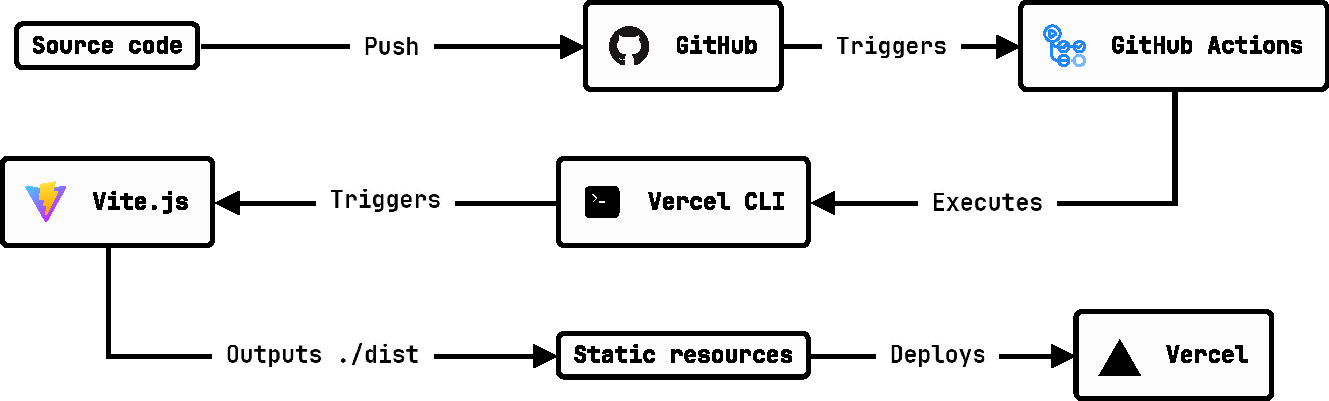
\includegraphics[max size={\linewidth}{\textheight}]{./assets/figures/deployment-diagram.pdf}
    \captionsetup{justification=centering}
    \caption[Diagram nasazení dokumentace]{Diagram nasazení dokumentace (diagram autora)}
    \label{fig:deployment}
\end{figure}

Průběh nasazení začíná dodáním kódu do GitHub repozitáře projektu.
Následně je možné manuálně spustit action\footnote{\url{https://github.com/features/actions}}, která pomocí \gls{cli} spustí na platformě Vercel \textit{build} a provede nasazení aplikace.
Vercel si stáhne nejnovější verzi kódu z GitHubu a provede build aplikace stejně jako v lokálním prostředí vývojáře.
Nasazená aplikace je dostupná skrze \gls{cdn} a je možné ji zobrazit v prohlížeči.
Vercel se stará o cachování a distribuci aplikace po celém světě~\cite{vercel-edge}.

\section{Distribuce knihovny}

JavaScriptové knihovny jsou distribuovány pomocí npm registry\footnote{\url{https://npmjs.com}}.
Pro distribuci je potřeba nadefinovat manifest soubor \texttt{package.json}\footnote{\url{https://docs.npmjs.com/cli/v10/configuring-npm/package-json}}, který obsahuje metadata o knihovně.

\begin{figure}[h]
    \centering
    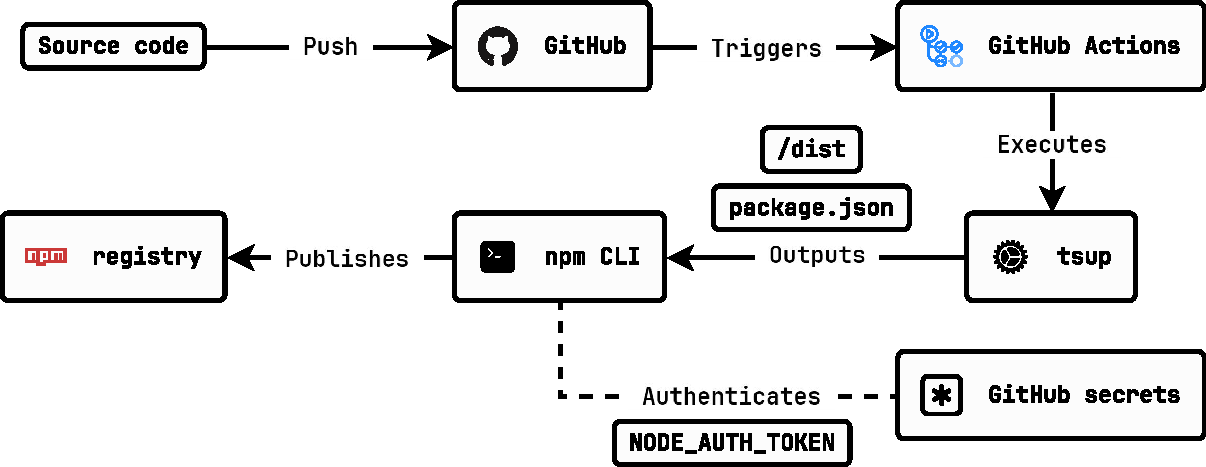
\includegraphics[max size={\linewidth}{\textheight}]{./assets/figures/deployment-library.pdf}
    \captionsetup{justification=centering}
    \caption[Diagram nasazení knihovny]{Diagram nasazení knihovny (diagram autora)}
    \label{fig:deployment-library}
\end{figure}

Důležitým krokem je připravit zdrojový kód k distribuci.
Pro tento účel jsem zvolil knihovnu \texttt{tsup}\footnote{\url{https://tsup.egoist.dev}}, která umožňuje jednoduše vytvořit balíček pro distribuci a to včetně TypeScript podpory a různých formátů modulů.

Knihovna je publikovaná pod názvem \texttt{solid-apg} a lze ji nainstalovat jedním z příkazů v ukázce~\ref{install-solid-apg}.

\begin{listing}[!ht]
    \begin{minted}{bash}
npm install solid-apg
# or
yarn add solid-apg
# or 
pnpm add solid-apg
# or
bun add solid-apg
\end{minted}
    \caption{Instalace knihovny solid-apg}
    \label{install-solid-apg}
\end{listing}
